

\begin{frame}{Processus}

\begin{columns}
  \column{0.38\linewidth}
\begin{figure}
    \centering
    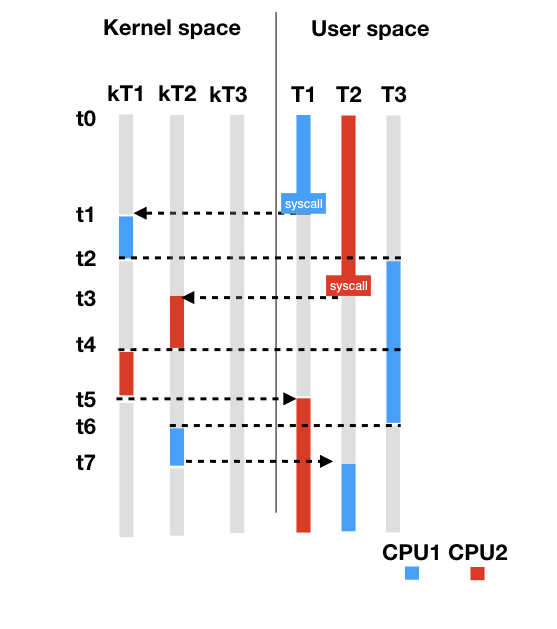
\includegraphics[width=\textwidth]{slides/images/scheduling.jpg}
\end{figure}

\column{0.58\linewidth}

\subtt{État d'un processus}

\begin{itemize}[label=$-$]
    \item Registres processeur
    \item Table des descripteurs fichiers
    \item Répertoire courant
    \item Variables d'environnement
\end{itemize}
\end{columns}

\end{frame}


\begin{frame}[fragile]{AST évolué}
    \begin{itemize}[leftmargin=-10pt] 
         \item
        \begin{lstlisting}
            type cmd_kind =
                | Internal of command (* les commandes precedentes *)
                | External of string list (* la triche avec execv *)
                | Cd of string (* getcwd / chdir *)
            type redirection =
                | In of string (* > *)
                | Out of string (* < *)
            type command = cmd_kind * redirection list
            type t = 
                | Command of command
                | Pipe of t * t (* | *)
                | And of t * t (* exit status *)
                | Or of t * t
            val execute : t -> unit
        \end{lstlisting}
    \end{itemize}

\end{frame}

\begin{frame}[fragile]{Nouvelle boucle de lecture}
\begin{lstlisting}
let minishell () =
 try
     Printf.printf "%s> %!" (Unix.getcwd ());
     while true do
       let cmd = input_line Stdlib.stdin in
       try 
         let cmd = Ast.parse cmd in
         let code = interprete cmd in
         Printf.printf "%s (%d)> %!" (Unix.getcwd ()) code
       with
       | Parser.Parsing_error err -> Parser.print_error err
       | Parser.Empty_line -> ()
     done
   with End_of_file -> ()
\end{lstlisting}
\end{frame}

\begin{frame}{}
    
\end{frame}

\begin{frame}{\texttt{cd}}
    
\end{frame}

\begin{frame}{\texttt{fork}}

\end{frame}
